% Results section

\[ To be reorganized \]

The results of the analysis are grouped into the type of band used to make each colour.  % More general notes about results

\subsection{Broad \& Broad Band Combinations}

\subsection{Broad \& Narrow Band Combinations}
Each broad and narrow band combination was tested against every broad-broad band combination that did not boarder the narrow band.

\subsubsection{UVW - U}
The UVW - U combination was tested clustered with the B-I, V-I, and B-V colours. % More general information about what we are looking for in this combination

\paragraph{Mean-Shift}
When clustered using Mean-Shift, a similar pattern of clustering was seen in all combinations.
Due to the structure of the Mean-Shift algorithm, it is drawn towards areas of high density in the distribution. % Refernce meanshift paper
Since the distribution of the UVW-U combinations were generally consentrated around zero in the colour-colour space, the Mean-Shift algorithm would pick out one large cluster with many smaller ones. 
Each smaller cluster had to be investigated to determine if the algorithm had found a meaningful cluster, or if it had just clustered noise.
In order to determine this, a cluster hierarchy was created with different bandwidth values to see how long each cluster lasted in the bandwidth space. 
If a small cluster was created at a low bandwidth level and stayed alive until the number of clusters became 2-3, then it is reasonable to assume that the cluster was meaningful.
Figure ~\ref{fig:UVWMS1} shows the result of one trial of Mean-Shift clustering with $h=0.6$ which created 4 clusters. 
Figure ~\ref{fig:UVWMS2} shows the result of one trial of Mean-Shift clustering with $h=0.4$, creating 10 clusters. 
The structure of cluster $2$ in both Figure ~ref{fig:UVWMS1} and Figure ~ref{fig:UVWMS2} can be seen distinctly. 
This cluster would have been viewed as noise if the hierarchy was not created, but after testing multiple bandwidth values, it can be seen that these objects are significant. 

\begin{figure}[H]
\centering
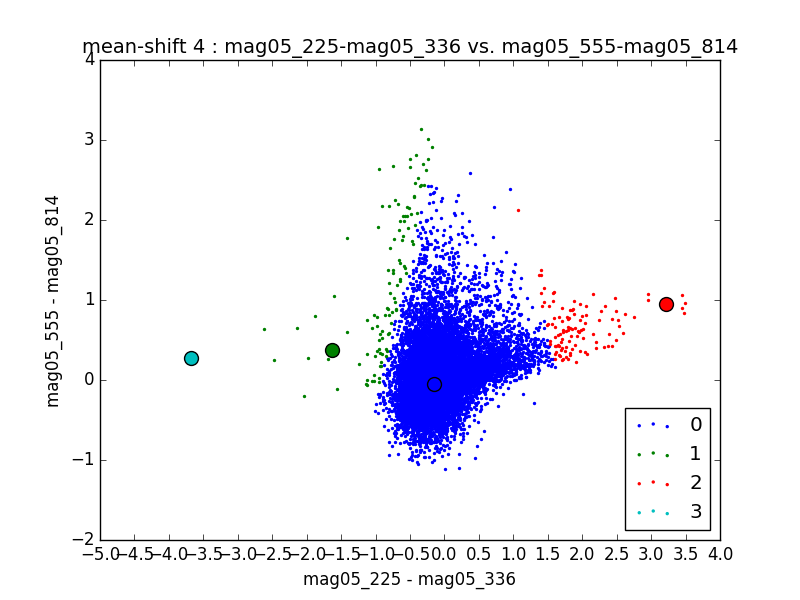
\includegraphics[width=\linewidth]{figs/meanshift_color_4cl_mag05_225-mag05_336vsmag05_555-mag05_814}
\caption{Colour-Colour distribution of the UVW-U and V-I colours, clustered using Mean-Shift with $h=0.6$. The colour of each point corresponds to the cluster the point was assigned to. Cluster numbers can be seen in the legend.}
\label{fig:UVWMS1}
\end{figure}

\begin{figure}[H]
\centering
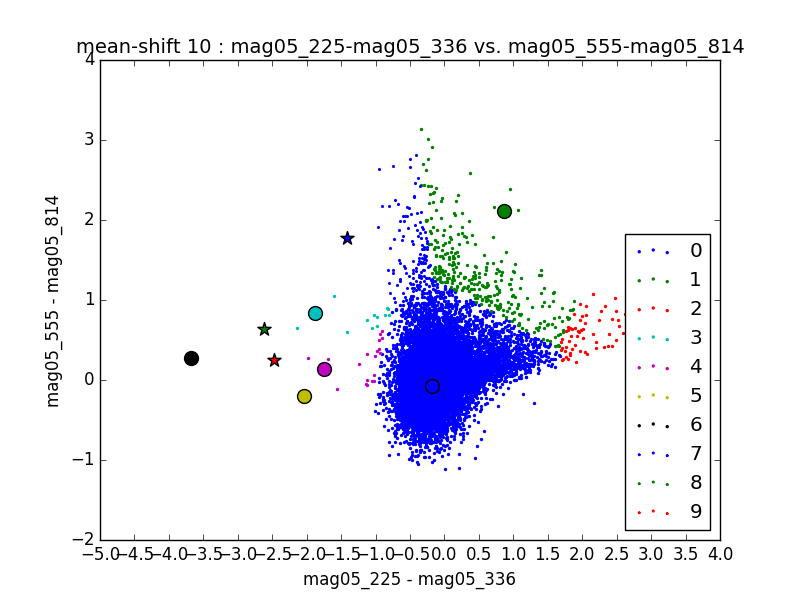
\includegraphics[width=\linewidth]{figs/meanshift_color_10cl_mag05_225-mag05_336vsmag05_555-mag05_814}
\caption{Colour-Colour distribution of the UVW-U and B-I colours, clustered using K-Means with $h=0.4$. The colour of each point corresponds to the cluster the point was assigned to. Cluster numbers can be seen in the legend.}
\label{fig:UVWMS2}
\end{figure}

\paragraph{K-Means}

When clustered using K-Means, two types of results were seen.
Figure ~\ref{fig:UVWKM1}, shows the result of K-Means clustering for $K=5$ against the B-V colour. 
\begin{figure}
\centering
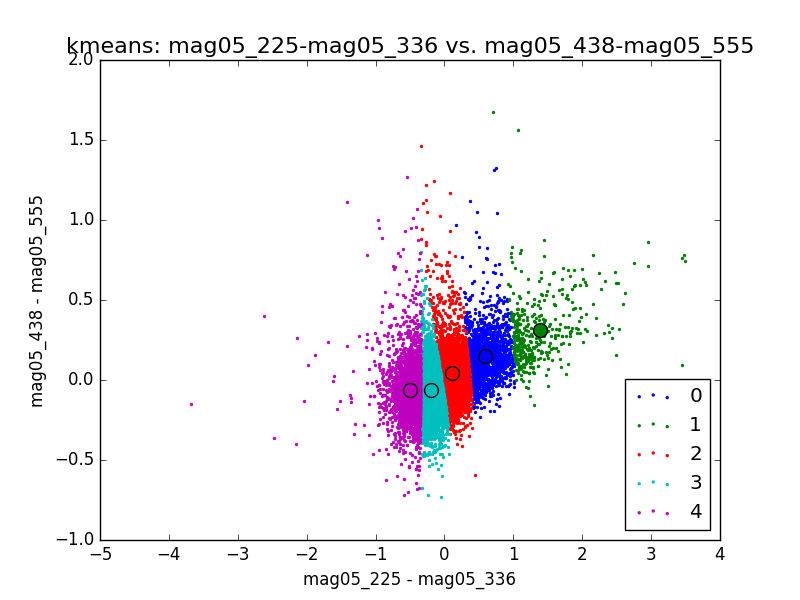
\includegraphics[width=\linewidth]{figs/kmeans_xy_5cl_mag05_225-mag05_336vsmag05_438-mag05_555}
\caption{Colour-Colour distribution of the UVW-U and B-V colours, clustered using K-Means with $K=5$. The colour of each point corresponds to the cluster the point was assigned to. Cluster numbers can be seen in the legend.}
\label{fig:UVWKM1}
\end{figure}
The algorithm split the data into groups based on its UVW - U colour. The pattern continued for all values of K, and the S Scores of the combination elbowed at $K=5$.
The second type of result for K-Means can be seen in Figure ~\ref{fig:UVWKM2}, against the B-I colour. 
This clustering segmented the data into circular groups within the distribution. 
Similar to the B-V combination, the S Score elbowed at $K=5$. 
When the objects were plotted on the whitelight image, both types of segmentation seemed to pick out objects that live in different structures of M83. % Reference Chandar
% Add test with CLAsPS score to show correlation with labels 
\begin{figure}[H]
\centering
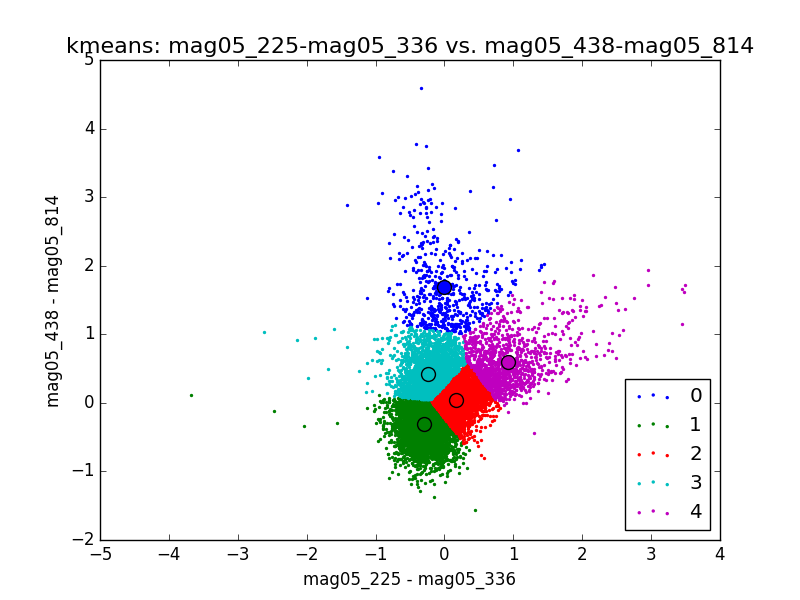
\includegraphics[width=\linewidth]{figs/kmeans_xy_5cl_mag05_225-mag05_336vsmag05_438-mag05_814}
\caption{Colour-Colour distribution of the UVW-U and B-I colours, clustered using K-Means with $K=5$. The colour of each point corresponds to the cluster the point was assigned to. Cluster numbers can be seen in the legend.}
\label{fig:UVWKM2}
\end{figure}

\subsubsection{U - OII}
The U - OII combination was clustered with the B-V, B-I, and V-I colours. % More general information about what we are looking for in this combination

\paragraph{Mean-Shift}
This colour seemed to be much more sensitive to bandwidth selection than other combinations.
With the B-V colour, $h=0.2$ produced $32$ clusters, while $h=0.4$ produced $3$. With the V-I colour, $h=0.35$ produced $17$ clusters, while $h=0.6$ produced $3$.
Due to this sensitivity, the bandwidth hierarchy was created on much narrower increases in $h$, which produced more meaningful clusters. 












